%\documentclass[12pt,notitlepage]{article}
\documentclass[a4paper,12pt]{article}
\usepackage[utf8]{inputenc}
\usepackage{graphicx}
\usepackage{verbatim}
\usepackage{amsthm}
\usepackage{amssymb}
\usepackage{pdfpages}
\usepackage{amsmath}
\usepackage{tikzsymbols}
\usepackage{mathtools}
\usepackage{enumitem}
\DeclarePairedDelimiter\ceil{\lceil}{\rceil}
\DeclarePairedDelimiter\floor{\lfloor}{\rfloor}

\usepackage{hyperref}
%\usepackage[T1]{fontenc}
\usepackage{url}
\usepackage{lipsum}
\usepackage{array}
\usepackage{multirow}
\usepackage{float}
\usepackage{lscape}
\usepackage{colortbl}
\newcolumntype{P}[1]{>{\centering\arraybackslash}p{#1}}
\usepackage[nottoc,numbib]{tocbibind}
\usepackage{fancyhdr}
\usepackage{hhline}
\usepackage[printonlyused]{acronym}

%\usepackage{txfonts}
\usepackage{lipsum,etoolbox}% http://ctan.org/pkg/{lipsum,etoolbox}
\usepackage{caption}
\usepackage{subcaption}

\usepackage{algorithm}
\usepackage[noend]{algpseudocode}

\makeatletter
\def\BState{\State\hskip-\ALG@thistlm}
\makeatother

\usepackage{minted}

\definecolor{black}{RGB}{0,0,0}

\usepackage{fancyvrb}

\usepackage{geometry}
\geometry{
	a4paper,
	total={170mm,257mm},
	right=3cm,
	left=3.5cm,
	top=3cm,
	bottom=3cm
}

\makeatletter
\DeclareRobustCommand{\rvdots}{%
	\vbox{
		\baselineskip4\p@\lineskiplimit\z@
		\kern-\p@
		\hbox{.}\hbox{.}\hbox{.}
}}
\makeatother
\usepackage{titlesec}
\usepackage{hyperref}
\titleclass{\subsubsubsection}{straight}[\subsection]

\newcounter{subsubsubsection}[subsubsection]
\renewcommand\thesubsubsubsection{\thesubsubsection.\arabic{subsubsubsection}}
\renewcommand\theparagraph{\thesubsubsubsection.\arabic{paragraph}} % optional; useful if paragraphs are to be numbered

\titleformat{\subsubsubsection}
{\normalfont\normalsize\bfseries}{\thesubsubsubsection}{1em}{}
\titlespacing*{\subsubsubsection}
{0pt}{3.25ex plus 1ex minus .2ex}{1.5ex plus .2ex}

\makeatletter
\renewcommand\paragraph{\@startsection{paragraph}{5}{\z@}%
	{3.25ex \@plus1ex \@minus.2ex}%
	{-1em}%
	{\normalfont\normalsize\bfseries}}
\renewcommand\subparagraph{\@startsection{subparagraph}{6}{\parindent}%
	{3.25ex \@plus1ex \@minus .2ex}%
	{-1em}%
	{\normalfont\normalsize\bfseries}}
\def\toclevel@subsubsubsection{4}
\def\toclevel@paragraph{5}
\def\toclevel@paragraph{6}
\def\l@subsubsubsection{\@dottedtocline{4}{7em}{4em}}
\def\l@paragraph{\@dottedtocline{5}{10em}{5em}}
\def\l@subparagraph{\@dottedtocline{6}{14em}{6em}}
\makeatother
\newcommand*\circled[1]{\tikz[baseline=(char.base)]{
		\node[shape=circle,draw,inner sep=2pt] (char) {#1};}}


\setcounter{secnumdepth}{4}
\setcounter{tocdepth}{4}
\newcommand{\und}{\underline{\hspace{.10in}}}
\begin{document}
	\begin{titlepage}
		\begin{center}
			\vspace*{9em}
			\Huge 
			MH4920\\ Supervised Independent Study I\\
			\vspace*{4em}
			\LARGE
			\textbf{String Format Vulnerability}\\		
			\vspace{4em}
			\textbf{Brandon Goh Wen Heng}\\
			\vspace*{4em}
			Academic Year 2017/18
			\vfill
		\end{center}
	\end{titlepage}
	
	\pagenumbering{roman}
	\tableofcontents
	\newpage
	\pagenumbering{arabic}
	\section{Introduction}
	An uncontrolled format string is an vulnerability where the user input can be used to inject malicious code read from an arbitrary memory region or to crash a program. This vulnerability stems from the use of the print symbols \texttt{\%s}, \texttt{\%x} and \texttt{\%n} as languages such as \texttt{C} are not type-safe. This will create an environment where the stack is popped multiple times, depending on the number of print symbols used and may reveal data in sensitive areas that are otherwise privileged.
	\section{Overview}
	This lab will look at a program that has the format string vulnerability and this lab will attempt to crash the program, view and write to regions that are otherwise inaccessible to the user.\\\\In particular, the following will be covered in each task:\\\\
	\circled{1} Crashing of the program\\\circled{2} Printing the value of \texttt{secret[1]} or \texttt{secret[2]}\\\circled{3} Modification of \texttt{secret[1]} or \texttt{secret[2]}\\\circled{4} Modification of \texttt{secret[1]} or \texttt{secret[2]} to a predetermined value
	\newpage
	\section{Vulnerability Exploit}
	\subsection{Generic Exploitation}
	This section will look into the exploitation of the given program \texttt{vul\_prog}. The code has been attached to the \hyperref[Appsec:3.1]{Appendix} for reference. The program has printed the address of the secrets for convenience sake but the detailed steps of obtaining the location of the secrets will be mentioned in this report for clarity and completeness.\\\\The program is first compiled and executed. The address is assumed to be hidden on the stack and can be found using \texttt{gdb}. Since the source code is known, we can determine the location of \texttt{secret} by using the command \texttt{p secret}.
	
\begin{figure}[H]
	\centering
	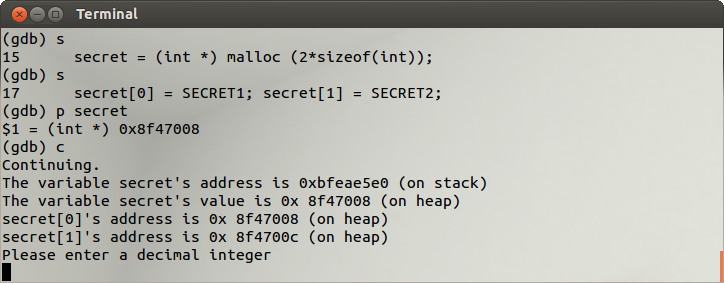
\includegraphics[width=0.9\linewidth]{varpos}
	\caption{\texttt{secret} array location}
	\label{fig:varpos}
\end{figure}
\noindent The address obtained can be checked against the address printed by the program. It is also important to note that the location obtained is the start of the \texttt{secret} array, or \texttt{secret}. To view the content of \texttt{secret[1]}, we note that the address offset is $+4$, this is because \texttt{sizeof(char)} is one but the array structure will pad the remaining 3 bytes to align against the machine word length (32 bits on a 32-bit machine). This will be looked into greater detail in the next few sections.\\\\\circled{1} Crashing of the program\\\\The use of \texttt{\%s} will treat the value in the stack as a pointer and will print the character to the location that it is pointing to. Similarly, \texttt{\%n} treats the value in the stack as a pointer but will instead overwrite of the memory address space it is pointing to. It is critical to understand that the program will crash when the pointer references a protected region, such as the kernel or an unassigned space. With this information, we can crash the program by using multiple \texttt{\%s} or \texttt{\%n} and hope that we get lucky.
\begin{figure}[H]
	\centering
	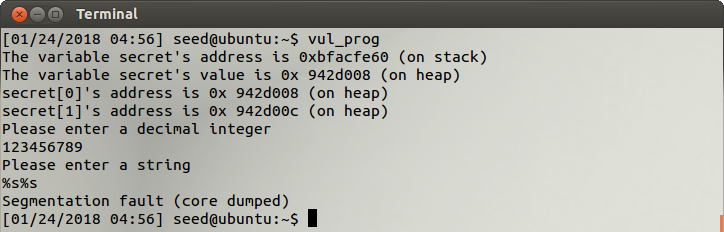
\includegraphics[width=0.9\linewidth]{strcrash}
	\caption{Crashed Program}
	\label{fig:strcrash}
\end{figure}
\noindent If the program is debugged using \texttt{gdb}, we will notice that the program crashes on the second \texttt{\%s} as the address that it happens to read from is \texttt{0x1}, which is protected. Therefore reading from that region will crash the program indefinitely.\\\\\circled{2} Printing the value of \texttt{secret[1]}\\\\To print out the value of \texttt{secret[1]}, we need to know the address and the number of print tokens to use. From before, we already know the address for the start of the array. We add the offset of $+4$ and it will point to \texttt{secret[1]}. To find out the number of print tokens to use, we will key in a random integer first and locate it on the stack. In the following figure, we input the value of $12349876$ and view the stack to find the appropriate value.
\begin{figure}[H]
	\centering
	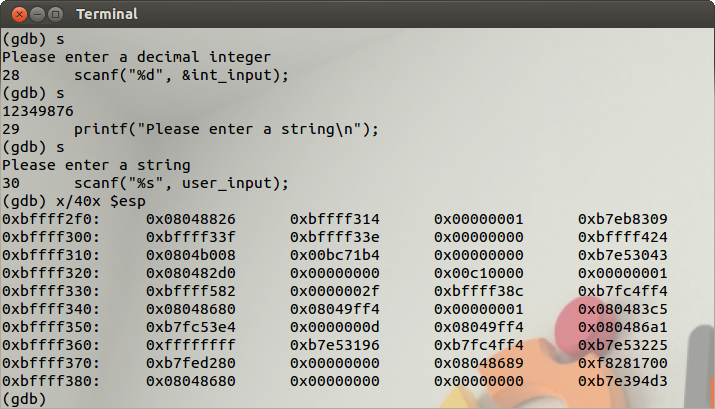
\includegraphics[width=0.9\linewidth]{espstrval}
	\caption{Search Stack Using \texttt{ESP}}
	\label{fig:espstrval}
\end{figure}
\noindent We note that the value of $12349876_{10}$ has the value of \texttt{0xbc71b4} in hex, which can easily be determined using a calculator. With reference to Figure 3, the relevant data can be found in address \texttt{0xbffff314}. We have also determined that eight \texttt{\%x} must be used followed by a \texttt{\%s}.
\begin{figure}[H]
	\centering
	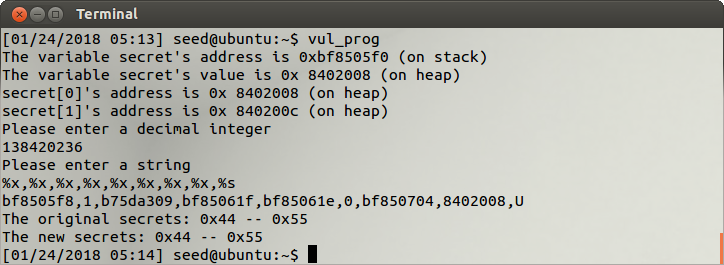
\includegraphics[width=0.9\linewidth]{sec1val}
	\caption{Printing \texttt{secret[1]} Value}
	\label{fig:sec1val}
\end{figure}
\noindent As we know the value of address of \texttt{secret[1]} now and the number of \texttt{\%x} to use, using it together will print out the secret in the last field. From Figure 4, the secret that is printed out has the value ``U''. Checking against the ASCII table, ``U'' has a hex value of \texttt{0x55} which corresponds to the secret that has been conveniently printed out by the program.\\\\\circled{3} Modification of \texttt{secret[1]}\\\\To modify \texttt{secret[1]}, we need to make use of the \texttt{\%n} command. The \texttt{\%n} allows the pointed address to be overwritten based on the number of characters that has been printed before it. Using this, we can change the value of \texttt{secret[1]}. To do so, we will use the same methods in \circled{2} but will use \texttt{\%n} instead of \texttt{\%s}. As it is not possible to modify the number of \texttt{\%x}, a technique of adjusting the text width can be used. In Figure 5, we have adjusted the text width to 8, to reflect 32-bit values in the memory. 
\begin{figure}[H]
	\centering
	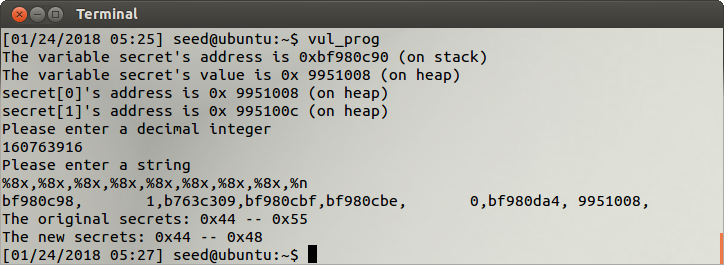
\includegraphics[width=0.9\linewidth]{sec1mod}
	\caption{Modification of \texttt{secret[1]}}
	\label{fig:sec1mod}
\end{figure}
\noindent We see from the output that the new secret has been modified when the \texttt{\%n} is used. In the next part, we will analyse further into changing the value to something that is predetermined.\\\\
\circled{4} Modification of \texttt{secret[1]} to a predetermined value\\\\The techniques used in \circled{3} will be used in this part. To set \texttt{secret[1]} to a specific value, we can use the text width of \texttt{\%x} to increase the value to be written into the memory. In our case, we would like to write the letter ``z'' into the memory, which has the hex value of \texttt{0x7a}. A hex value of \texttt{0x7a} corresponds to the decimal number 122 so this number of characters must be printed before \texttt{\%n} is called.
\begin{figure}[H]
	\centering
	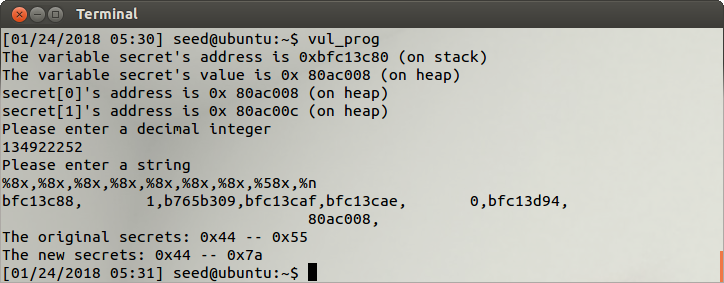
\includegraphics[width=0.9\linewidth]{sec1predmod}
	\caption{Modifying \texttt{secret[1]} To Predetermined Value}
	\label{fig:sec1predmod}
\end{figure}
\noindent From Figure 6, \texttt{\%8x,\%8x,\%8x,\%8x,\%8x,\%8x,\%8x,\%58x,\%n} is used. If we perform the calculations, we have seven \texttt{\%x} with a width of 8, one \texttt{\%x} with a width of 58 and eight ``,'' symbols. Adding all these up,
$$7\times 8+1\times 58+8=122$$
This gives us the required number to be overwritten and will be stored in the heap. Figure 6 shows that our method of overwriting has proven to be correct. Also, if the number that we would like to overwrite is less than the number of characters to be printed, for example a hex value of \texttt{0x2} but the number of \texttt{\%x} that must be used is 6, then we can use \texttt{\%hn}, \texttt{\%hhn} to write the last 2 bytes or 1 byte of the hex value respectively. We use this by forcing an overflow on the number of characters, which will act in the same manner as the \textit{modulo} function in mathematics.
\subsection{Exploitation Without Leading Input}
In the following section, address randomisation is turned off and the same attack repeated. It can be turned off via the following command,
\begin{verbatim}
# sysctl -w kernel.randomize_va_space=0
\end{verbatim}
After disabling address randomisation, the address on the stack and heap remain unchanged after multiple executions, which can also be seen in Figure 7.
\begin{figure}[H]
	\centering
	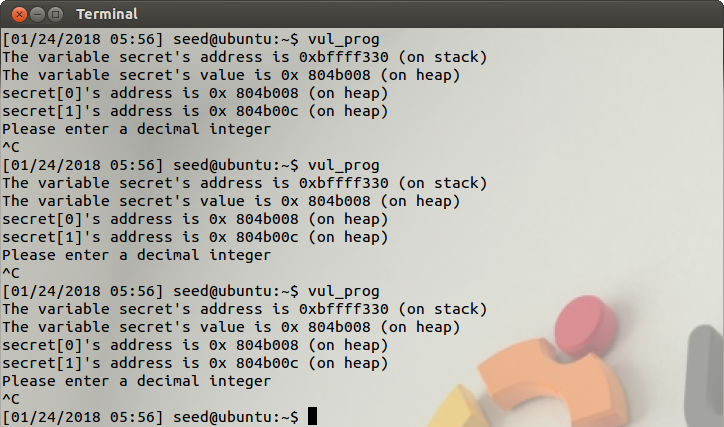
\includegraphics[width=0.9\linewidth]{ncadd}
	\caption{No Change in Address}
	\label{fig:ncadd}
\end{figure}
\noindent 
The removal of the leading integer input complicates the attack as hex values cannot be typed through \texttt{STDIN} and requires the reading of an external file. The code for the writing of this file has been attached to the \hyperref[Appsec:3.2]{Appendix}. As \texttt{secret[1]} is in the address with address ending with the byte \texttt{0x0c}, this corresponds to the new page command when used with \texttt{scanf}. Due to this problem, we dynamically add an extra element to the \texttt{secret} array by increasing the number of \texttt{malloc} used. To ensure that we do not edit or view the contents of the incorrect index, \texttt{secret[2]} is set with the hex value of \texttt{0x66}.
\\\\\circled{1} Crashing of the program\\\\Crashing of the program works in the same way as the previous task and will require only two \texttt{\%s} to be used as the second address being printed is \texttt{0x1} again, which is protected.\\\\\circled{2} View the contents of \texttt{secret[2]}\\\\The address of \texttt{secret[2]} is calculated by using the offset of $+8$ from the address of \texttt{secret}. Using \texttt{gdb}, it can be noticed that the changes performed on the vulnerable program code will require 1 additional \texttt{\%x}. It is similarly followed by a \texttt{\%s}. In our case, the address of \texttt{secret[0]} is \texttt{0x804b008} so \texttt{secret[2]} will be located at the address \texttt{0x804b010}.
\begin{figure}[H]
	\centering
	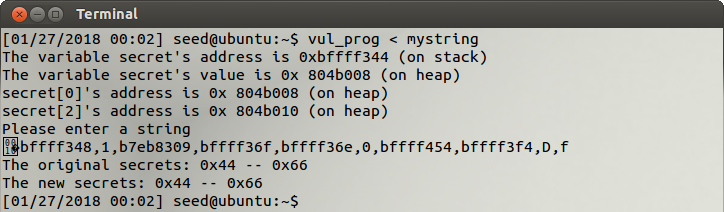
\includegraphics[width=0.9\linewidth]{viewadd2}
	\caption{Printing \texttt{secret[2]}}
	\label{fig:viewadd2}
\end{figure}
\noindent From Figure 8, it can be noticed that the second \texttt{\%s} prints out the value of \texttt{secret[2]} as it is the tenth print token. The letter ``f'' corresponds to the hex value \texttt{0x66}, which is what has been printed out by the program.\\\\
\circled{3} \& \circled{4} Modification of \texttt{secret[2]}\\\\The steps to perform modification are again similar to task 1, where the \texttt{\%s} is replaced with a \texttt{\%n} instead. When executing the program this time, the number of characters being printed is less than the original secret and will make it easier for us to view the modifications.
\begin{figure}[H]
	\centering
	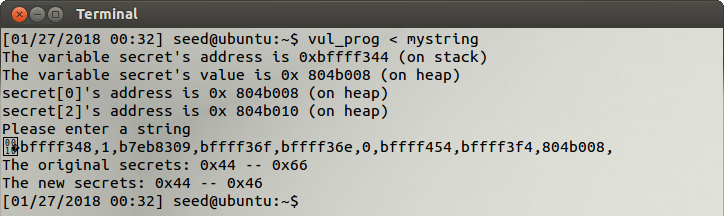
\includegraphics[width=0.9\linewidth]{sec2mod}
	\caption{Modification of \texttt{secret[2]}}
	\label{fig:sec2mod}
\end{figure}

	\newpage
	\section{Appendix}
	\subsection{Vulnerable Program: \texttt{vul\_prog.c}}
	\begin{minted}{C}
/*vul_prog.c*/
#include <stdio.h>
#include <stdlib.h>
#define SECRET1 0x44
#define SECRET2 0x55

int main(int argc,char *argv[])
{
    char user_input[100];
    int *secret;
    int int_input;
    int a,b,c,d;

    /*Secret stored on heap*/
    secret=(int *)malloc(3*sizeof(int));

    /*Getting secret*/
    secret[0]=SECRET1; secret[1]=SECRET2;
    printf("The variable secret's address is 0x%8x (on stack)\n", 
    (unsigned int)&secret);
    printf("The variable secret's value is 0x%8x (on heap)\n", 
    (unsigned int)secret);
    printf("secret[0]'s address is 0x%8x (on heap)\n", 
    (unsigned int)&secret[0]);
    printf("secret[2]'s address is 0x%8x (on heap)\n", 
    (unsigned int)&secret[2]);

    /*Get input from user*/
    printf("Please enter a decimal integer\n");
    scanf("%d", &int_input);
    printf("Please enter a string\n");
    scanf("%s", user_input);

    /*Vulnerable place*/
    printf(user_input);
    printf("\n");

    /*Verify whether attack is successful*/
    printf("The original secrets: 0x%x -- 0x%x\n", SECRET1, SECRET2);
    printf("The new secrets: 0x%x -- 0x%x\n", secret[0], secret[1]);
    return 0;
}
\end{minted}
\newpage
\subsection{Input File: \texttt{mystring}}
\label{Appsec:3.2}
\begin{minted}{C}
#include <stdio.h>
#include <string.h>
#include <sys/stat.h>
#include <fcntl.h>

int main()
{
    char buf[1000];
    int fp, size;
    unsigned int *address;
    
    /* Address to put at front of file*/
    address = (unsigned int *) buf;
    *address = 0x0804b010;
    
    /*Input for rest of string*/
    scanf("%s", buf+4);
    size = strlen(buf+4) + 4;
    printf("The string length is %d\n", size);
    
    /*Writing buf to file "mystring"*/
    fp = open("mystring", O_RDWR | O_CREAT | O_TRUNC,
    S_IRUSR | S_IWUSR);
    if (fp != -1) {
        write(fp, buf, size);
        close(fp);
    } else {
        printf("Open failed!\n");
    }
}
\end{minted}
\end{document}